\begin{enumerate}[label=\thesection.\arabic*,ref=\thesection.\theenumi]
\item Find the angle between two vectors $\overrightarrow{a}$ and $\overrightarrow {b} $ with magnitudes $\sqrt{3}$ and 2 respectively having $\overrightarrow {a}.\overrightarrow {b}=\sqrt{6}$.
	\\
	\solution
		\iffalse
\documentclass[10pt]{article}
\usepackage{graphicx}
\usepackage[none]{hyphenat}
\usepackage{graphicx}
\usepackage{listings}
\usepackage[english]{babel}
\usepackage{siunitx}
\usepackage{graphicx}
\usepackage{caption} 
\usepackage{booktabs}
\usepackage{array}
\usepackage{amssymb} % for \because
\usepackage{amsmath}   % for having text in math mode
\usepackage{extarrows} % for Row operations arrows
\usepackage{listings}
\usepackage[utf8]{inputenc}
\lstset{
  frame=single,
  breaklines=true
}
\usepackage{hyperref}
  
%Following 2 lines were added to remove the blank page at the beginning
\usepackage{atbegshi}% http://ctan.org/pkg/atbegshi
\AtBeginDocument{\AtBeginShipoutNext{\AtBeginShipoutDiscard}}


%New macro definitions
\newcommand{\mydet}[1]{\ensuremath{\begin{vmatrix}#1\end{vmatrix}}}
\providecommand{\brak}[1]{\ensuremath{\left(#1\right)}}
\newcommand{\solution}{\noindent \textbf{Solution: }}
\newcommand{\myvec}[1]{\ensuremath{\begin{pmatrix}#1\end{pmatrix}}}
\providecommand{\norm}[1]{\left\lVert#1\right\rVert}
\providecommand{\abs}[1]{\left\vert#1\right\vert}
\let\vec\mathbf{}
\begin{document}

\begin{center}
\title{\textbf{VECTORS}}
\date{\vspace{-5ex}} %Not to print date automatically
\maketitle
\end{center}

\section{12$^{th}$ Maths - EXERCISE-10.3}

\begin{enumerate}
\item Find the angle between two vectors $\overrightarrow{a}$ and $\overrightarrow {b} $ with magnitudes $\sqrt{3}$ and 2 respectively having $\overrightarrow {a}.\overrightarrow {b}=\sqrt{6}$.\\  

\solution
\fi
From the given information,
\begin{align}
\norm{\vec{a}}&=\sqrt{3}\\
\norm{\vec{b}}&= 2\\
{\vec{a}^{\top}}{\vec{b}}&=\sqrt{6}  
\end{align}
Thus,
\begin{align}
\cos\theta&=\frac{{\vec{a}^{\top}}{\vec{b}}}{\norm{\vec{a}}\norm{\vec{b}}}\\
&=\frac{1}{\sqrt{2}}\\
\implies\theta&={45}\degree
\end{align}

\item Find the angle between the the vectors $\hat{i}-2\hat{j}+3\hat{k}$ and $3\hat{i}-2\hat{j}+\hat{k}$.
	\\
	\solution
		\iffalse
\documentclass[journal,12pt]{article}
\usepackage{graphicx}
\usepackage[none]{hyphenat}
\usepackage{graphicx}
\usepackage{listings}
\usepackage[english]{babel}
\usepackage{siunitx}
\usepackage{graphicx}
\usepackage{caption} 
\usepackage{booktabs}
\usepackage{array}
\usepackage{amssymb} % for \because
\usepackage{amsmath}   % for having text in math mode
\usepackage{extarrows} % for Row operations arrows
\usepackage{listings}
\usepackage[utf8]{inputenc}
\lstset{
  frame=single,
  breaklines=true
}
\usepackage{hyperref}
  
%Following 2 lines were added to remove the blank page at the beginning
\usepackage{atbegshi}% http://ctan.org/pkg/atbegshi
\AtBeginDocument{\AtBeginShipoutNext{\AtBeginShipoutDiscard}}


%New macro definitions
\newcommand{\mydet}[1]{\ensuremath{\begin{vmatrix}#1\end{vmatrix}}}
\providecommand{\brak}[1]{\ensuremath{\left(#1\right)}}
\newcommand{\solution}{\noindent \textbf{Solution: }}
\newcommand{\myvec}[1]{\ensuremath{\begin{pmatrix}#1\end{pmatrix}}}
\providecommand{\norm}[1]{\left\lVert#1\right\rVert}
\providecommand{\abs}[1]{\left\vert#1\right\vert}
\let\vec\mathbf

\begin{document}

\begin{center}
\title{\textbf{VECTORS}}
\date{\vspace{-5ex}} %Not to print date automatically
\maketitle
\end{center}

\section*{$12^{th}$ Maths - EXERCISE-10.3}

\begin{enumerate}
\item Find the angle between the vectors $\\ \overrightarrow{a}=\hat{i}-2\hat{j}+3\hat{k}$ and $\overrightarrow{b}=3\hat{i}-2\hat{j}+\hat{k}$  
\section*{solution}
\fi
Let the given points be
\begin{align}
	\vec{a} &= \myvec{1\\-2\\3} , \vec{b} = \myvec{3\\ -2 \\ 1},
\end{align}
Since 
\begin{align}
\vec{a}^{\top}\vec{b}=10, \,
\norm{\vec{a}}=\sqrt{14}, \, 
	\norm{\vec{b}}&=\sqrt{14}, 
\label{eq:chapters/12/10/3/2/5}
\\
\cos\theta=\frac{\vec{a}^{\top}\vec{b}}{\norm{\vec{a}}\norm{\vec{b}}}
	&= \frac{5}{7}
	\\
	\implies \theta&= \cos^{-1}\frac{5}{7}
\end{align}

\item Find the projection of the vector $\hat{i}-\hat{j}$ on the vector $\hat{i}+\hat{j}$.
	\\
		\iffalse
\documentclass[12pt]{chapters/10/7/4/3/figsarticle}
\usepackage{graphicx}
\usepackage[none]{chapters/10/7/4/3/figshyphenat}
\usepackage{graphicx}
\usepackage{listings}
\usepackage[english]{chapters/10/7/4/3/figsbabel}
\usepackage{graphicx}
\usepackage{caption} 
\usepackage{booktabs}
\usepackage{array}
\usepackage{amssymb} % for \because
\usepackage{amsmath}   % for having text in math mode
\usepackage{extarrows} % for Row operations arrows
\usepackage{listings}
\lstset{
  frame=single,
  breaklines=true
}
\usepackage{hyperref}
  
%Following 2 lines were added to remove the blank page at the beginning
\usepackage{atbegshi}% http://ctan.org/pkg/atbegshi
\AtBeginDocument{\AtBeginShipoutNext{\AtBeginShipoutDiscard}}


%New macro definitions
\newcommand{\mydet}[1]{chapters/10/7/4/3/figs\ensuremath{\begin{vmatrix}#1\end{vmatrix}}}
\providecommand{\brak}[1]{chapters/10/7/4/3/figs\ensuremath{\left(#1\right)}}
\newcommand{\solution}{\noindent \textbf{Solution: }}
\newcommand{\myvec}[1]{chapters/10/7/4/3/figs\ensuremath{\begin{pmatrix}#1\end{pmatrix}}}
\providecommand{\norm}[1]{chapters/10/7/4/3/figs\left\lVert#1\right\rVert}
\providecommand{\abs}[1]{chapters/10/7/4/3/figs\left\vert#1\right\vert}
\let\vec\mathbf


\begin{document}

\begin{center}
\title{\textbf{VECTORS}}
\date{\vspace{-5ex}} %Not to print date automatically
\maketitle
\end{center}

\setcounter{page}{1}

\section{10$^{th}$ Maths - Chapter 10}

This is Problem-3 from Exercise 10.3

\begin{enumerate}
\item Find the projection of the vector $\hat{i}-\hat{j}$ on the vector $\hat{i}+\hat{j}$  
\end{enumerate}
\section{SOLUTION}
\fi
\solution
The given points are
\begin{align}
 \vec{A}=\myvec{1\\ -1},
 \vec{B}=\myvec{1\\ 1}
\end{align}
Since
\begin{align}
	\vec{A}^\top \vec{B} &= \myvec{1 &-1} \myvec{1\\ 1}=\myvec{1 \times 1}+\myvec{-1 \times  1}=0
	\\
	\norm {\vec {B}}^2 &= (\vec{B}^\top  \vec{B})=\myvec{1 & 1} \myvec{1\\ 1}= (1 \times  1)+(1 \times  1)=2,
\end{align}
and the project vector is given by 
\begin{align}
	\vec{C} &= 
	\frac{\vec{A}^\top  \vec{B}}{\norm {\vec{B}}}^2 \vec{B}
	&=\frac{0}{2} \myvec{1\\ 1}
	=\myvec{0\\ 0}
\end{align}
This is verfied in Fig.
		\ref{fig:12/10/3/3Figure}.
\begin{figure}[h]
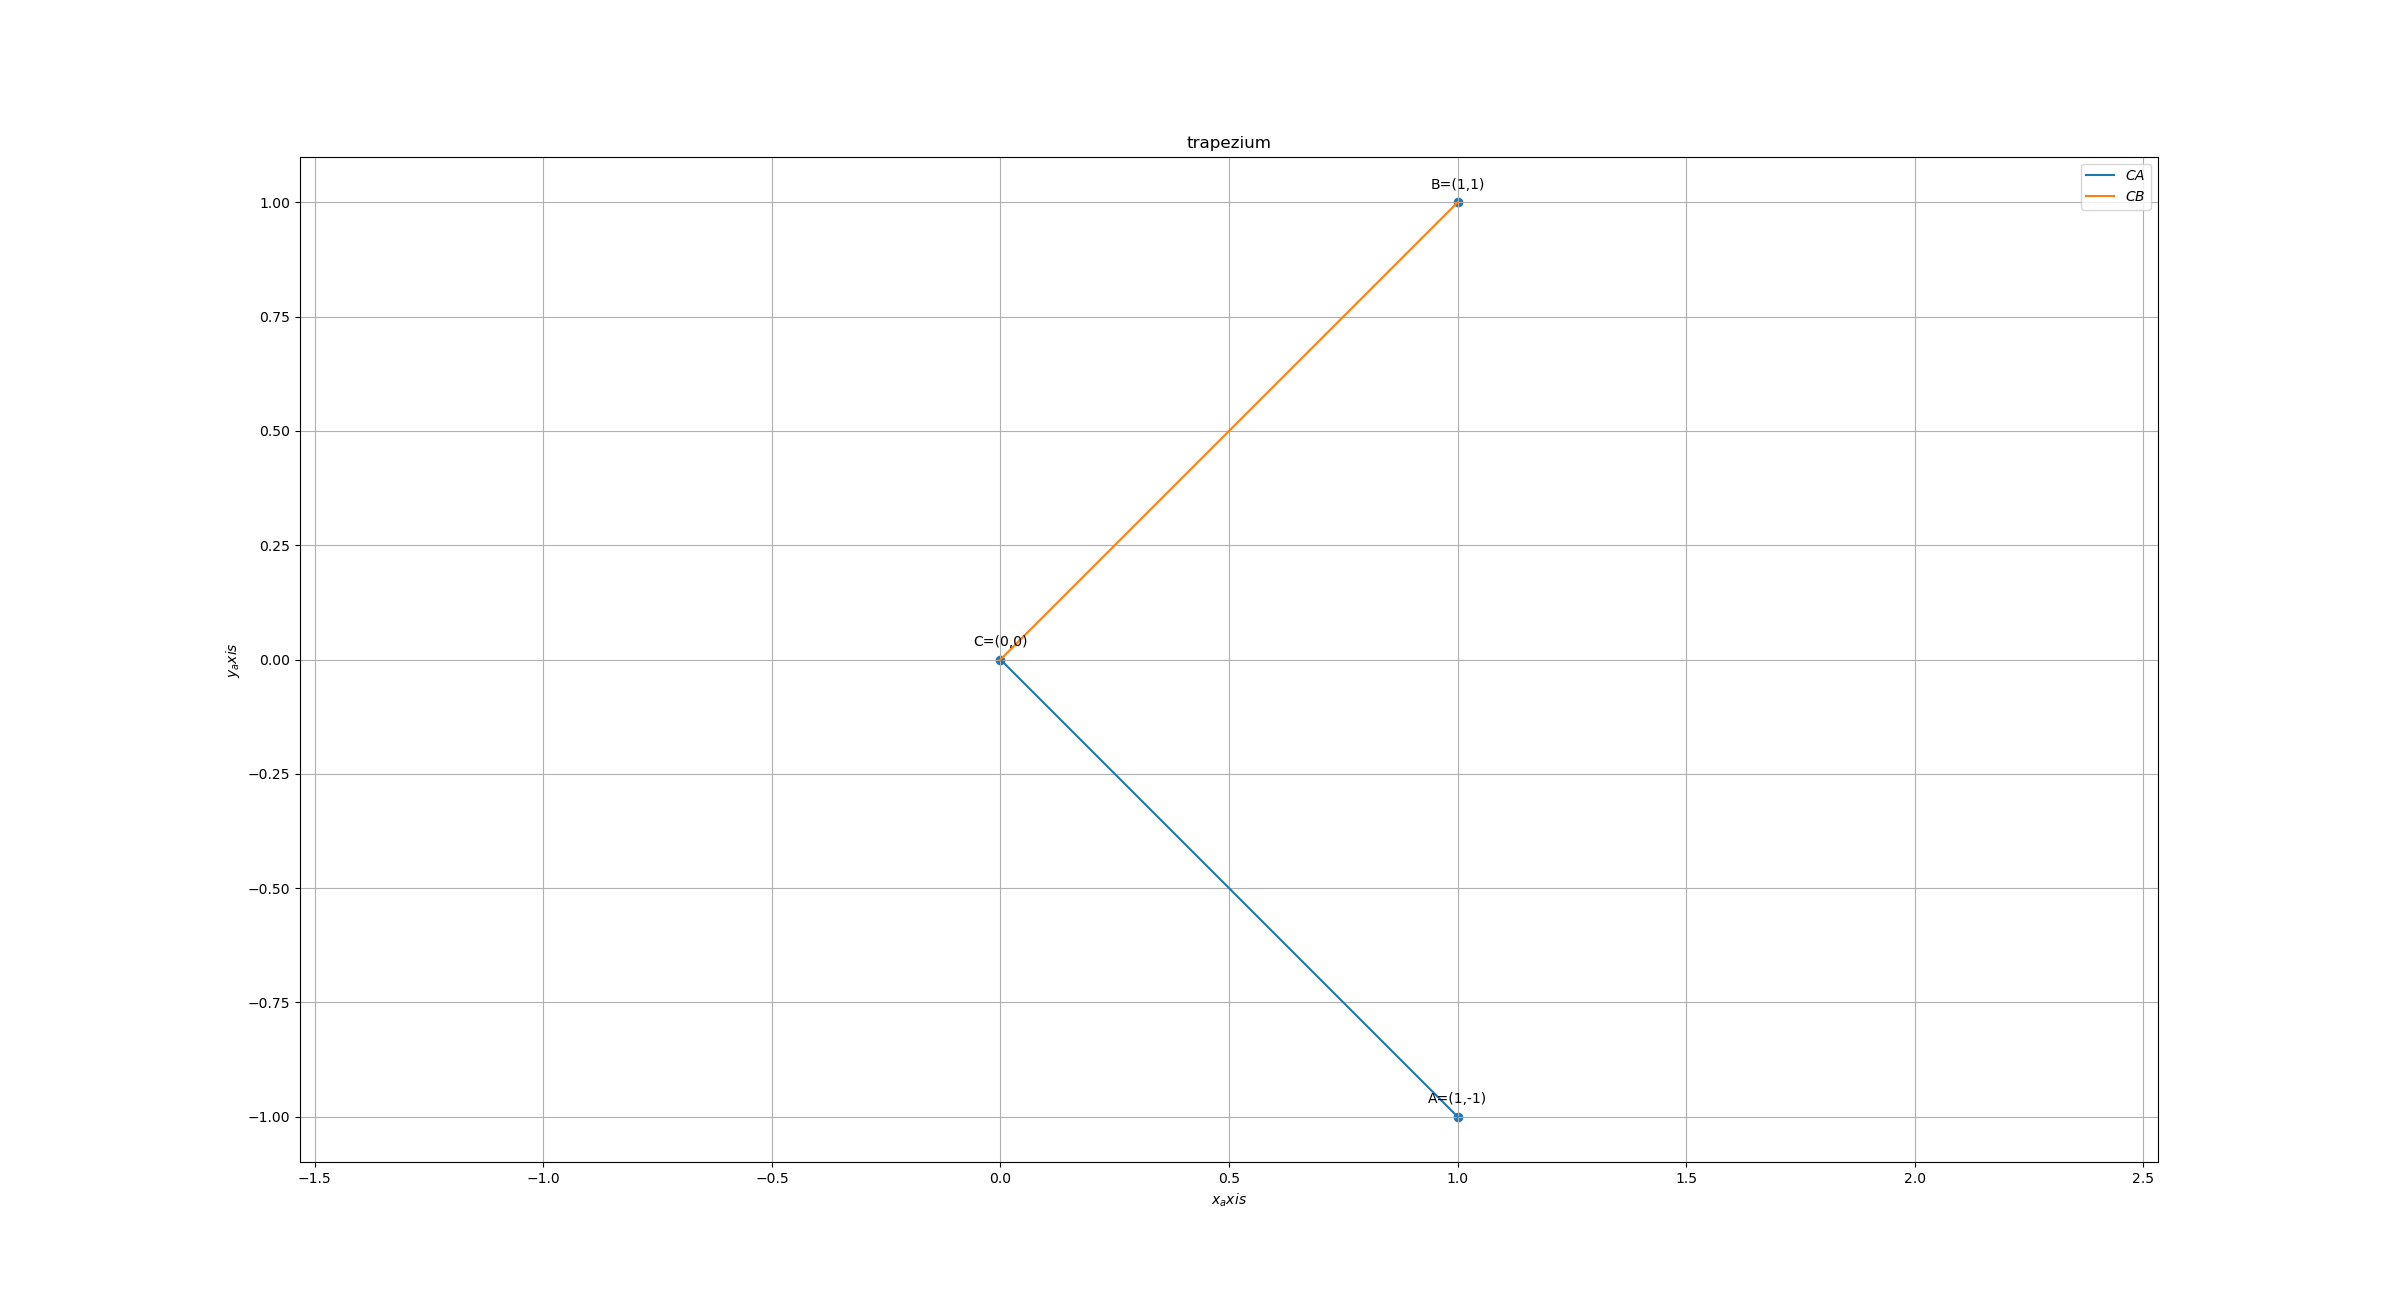
\includegraphics[width=\columnwidth]{chapters/12/10/3/3/figs/vector.png}
\caption{}
		\label{fig:12/10/3/3Figure}
\end{figure}

\item Find the projection of the vector $\hat{i}+3\hat{j}+7\hat{k}$ on the vector $7\hat{i}-\hat{j}+8\hat{k}$.
	\\
	\solution
		\iffalse
\documentclass[12pt]{article}
\usepackage{graphicx}
%\documentclass[journal,12pt,twocolumn]{IEEEtran}
\usepackage[none]{hyphenat}
\usepackage{graphicx}
\usepackage{listings}
\usepackage[english]{babel}
\usepackage{graphicx}
\usepackage{caption}
\usepackage[parfill]{parskip}
\usepackage{hyperref}
\usepackage{booktabs}
\usepackage{amsmath}
%\usepackage{setspace}\doublespacing\pagestyle{plain}
\def\inputGnumericTable{}
\usepackage{color}                                            %%
    \usepackage{array}                                            %%
    \usepackage{longtable}                                        %%
    \usepackage{calc}                                             %%
    \usepackage{multirow}                                         %%
    \usepackage{hhline}                                           %%
    \usepackage{ifthen}
\usepackage{array}
\usepackage{amsmath}   % for having text in math mode
\usepackage{parallel,enumitem}
\usepackage{listings}
\lstset{
language=tex,
frame=single,
breaklines=true
}
 
%Following 2 lines were added to remove the blank page at the beginning
\usepackage{atbegshi}% http://ctan.org/pkg/atbegshi
\AtBeginDocument{\AtBeginShipoutNext{\AtBeginShipoutDiscard}}
%
%New macro definitions
\newcommand{\mydet}[1]{\ensuremath{\begin{vmatrix}#1\end{vmatrix}}}
\providecommand{\brak}[1]{\ensuremath{\left(#1\right)}}
\providecommand{\norm}[1]{\left\lVert#1\right\rVert}
\newcommand{\solution}{\noindent \textbf{Solution: }}
\newcommand{\myvec}[1]{\ensuremath{\begin{pmatrix}#1\end{pmatrix}}}
\let\vec\mathbf
\begin{document}
\begin{center}
\enlargethispage{-4cm}
\title{\textbf{VECTOR ALGEBRA}}
\date{\vspace{-5ex}} %Not to print date automatically
\maketitle
\end{center}
\setcounter{page}{1}
\section*{12$^{th}$ Maths - Chapter 10}
This is Problem-4 from Exercise 10.3
\begin{enumerate}
	\item Find the projection of the vector $\hat{i}+3\hat{j}+7\hat{k}$ on the vector $7\hat{i}-\hat{j}+8\hat{k}$.

\solution 
\fi
		Let 
\begin{align}
 \vec{A} =\myvec{1\\3\\7}, \vec{B} =\myvec{7\\-1\\8}
\end{align}
The desired projection  is given by
\begin{align}
	\vec{C}=\frac{\Vec{A}^\top \Vec{B}}{\norm{\vec{B}}^2}\vec{B}\label{eq:chapters/12/10/3/4/2}
	  =\frac{\myvec{1 & 3 & 7}\myvec{7\\-1\\8}}{2}\myvec{7\\-1\\8}
		=\frac{10}{19}\myvec{7\\-1\\8}
 \end{align}

\item Show that each of the given three vectors is a unit vector: 

 $\frac{1}{7}(2\hat{i}+3\hat{j}+6\hat{k}),\frac{1}{7}(3\hat{i}-6\hat{j}+2\hat{k}),\frac{1}{7}(6\hat{i}+2\hat{j}-3\hat{k}$)
 
Also,show that they are mutually perpendicular to each other.
	\\
	\solution
		\iffalse
\documentclass[journal,12pt,twocolumn]{IEEEtran}
\usepackage{graphicx}
\graphicspath{{./figs/}}{}
\usepackage{amsmath,amssymb,amsfonts,amsthm}
\newcommand{\myvec}[1]{\ensuremath{\begin{pmatrix}#1\end{pmatrix}}}
\providecommand{\norm}[1]{\lVert#1\rVert}
\usepackage{listings}
\usepackage{watermark}
\usepackage{titlesec}
\usepackage{caption}
\let\vec\mathbf
\lstset{
frame=single, 
breaklines=true,
columns=fullflexible
}
\thiswatermark{\centering \put(0,-105.0){
\includegraphics[scale=0.15]{/sdcard/IITH/vectors/12.10.3.5/figs/logo.png}} }
\title{\mytitle}
\title{
Assignment - 12.10.3.5
}
\author{Surajit Sarkar}
\begin{document}
\maketitle
\tableofcontents
\bigskip
\section{\textbf{Problem}}
Show that each of the given three vectors is a unit vector:$\frac{1}{7}\myvec{2\hat{i}+3\hat{j}+6\hat{k}},\frac{1}{7}\myvec{3\hat{i}-6\hat{j}+2\hat{k}},\frac{1}{7}\myvec{6\hat{i}+2\hat{j}-3\hat{k}}$
Also, Show that they are mutually perpendicular to eatch other.
\section{\textbf{Solution}}
\fi
Let
\begin{align}
\vec{A}=\myvec{\frac{2}{7}\\ \frac{3}{7}\\ \frac{6}{7}},\Vec{B}=\myvec{\frac{3}{7}\\ -\frac{6}{7}\\ \frac{2}{7}},\vec{C}=\myvec{\frac{6}{7}\\ \frac{2}{7}\\ -\frac{3}{7}}
\end{align}
Then
\begin{align}
	\norm{\vec{A}}
=
\norm{\vec{B}}
=
\norm{\vec{C}}
=1
\end{align}
Also,
\begin{align}
\vec{A}^{\top}\vec{B}&=\myvec{\frac{2}{7}&\frac{3}{7}&\frac{6}{7}}\myvec{\frac{3}{7}\\-\frac{6}{7}\\ \frac{2}{7}}
=\frac{6}{49}-\frac{18}{49}+\frac{12}{49}
=0
\\
\vec{B}^{\top}\vec{C}&=\myvec{\frac{3}{7}&-\frac{6}{7}&\frac{2}{7}}\myvec{\frac{6}{7}\\ \frac{2}{7}\\-\frac{3}{7}}
=\frac{18}{49}-\frac{12}{49}-\frac{6}{49}
=0
\\
\vec{C}^{\top}\vec{A}&=\myvec{\frac{6}{7}&\frac{2}{7}&-\frac{3}{7}}\myvec{\frac{2}{7}\\ \frac{3}{7}\\ \frac{6}{7}}
=\frac{12}{49}+\frac{6}{49}-\frac{18}{49}
=0
\end{align}


\item Find $\abs{\overrightarrow {a}}$ and $\abs{\overrightarrow {b}}$,if ($\overrightarrow {a}+\overrightarrow {b}).(\overrightarrow {a}-\overrightarrow {b})=8$ and $\abs{\overrightarrow {a}}=8\abs{\overrightarrow {b}}$.
\item Evaluate the product(3$\overrightarrow {a}-5\overrightarrow {b}).(2\overrightarrow {a}+7\overrightarrow {b}$).
\item Find the magnitude of two vectors $\overrightarrow {a}$ and $\overrightarrow {b}$, having the same magnitude and such that the angle between them is $60\degree$ and their scalar product is $\frac{1}{2}$
\item Find $\abs{\overrightarrow {x}}$,if for a unit vector $\overrightarrow {a},(\overrightarrow {x}-\overrightarrow {a}).(\overrightarrow {x}+\overrightarrow {a}$)=12.
	\\
		\iffalse
\documentclass[12pt]{article}
\usepackage{graphicx}
%\documentclass[journal,12pt,twocolumn]{IEEEtran}
\usepackage[none]{hyphenat}
\usepackage{graphicx}
\usepackage{listings}
\usepackage[english]{babel}
\usepackage{graphicx}
\usepackage{caption} 
\usepackage{hyperref}
\usepackage{booktabs}
\usepackage{array}
\usepackage{amsmath}   % for having text in math mode
\usepackage{listings}
\lstset{
  frame=single,
  breaklines=true
}
  
%Following 2 lines were added to remove the blank page at the beginning
\usepackage{atbegshi}% http://ctan.org/pkg/atbegshi
\AtBeginDocument{\AtBeginShipoutNext{\AtBeginShipoutDiscard}}
%


%New macro definitions
\newcommand{\mydet}[1]{\ensuremath{\begin{vmatrix}#1\end{vmatrix}}}
\providecommand{\brak}[1]{\ensuremath{\left(#1\right)}}
\providecommand{\norm}[1]{\left\lVert#1\right\rVert}
\newcommand{\solution}{\noindent \textbf{Solution: }}
\newcommand{\myvec}[1]{\ensuremath{\begin{pmatrix}#1\end{pmatrix}}}
\let\vec\mathbf

\begin{document}

\begin{center}
\title{\textbf{Vector Dot Product}}
\date{\vspace{-5ex}} %Not to print date automatically
\maketitle
\end{center}
\setcounter{page}{1}

\section{12$^{th}$ Maths - Chapter 10}
This is Problem-9 from Exercise 10.3
\begin{enumerate}
\item Find $\norm{\vec{x}}$, if for a unit vector $\vec{a}$, $\brak{\vec{x}-\vec{a}}.\brak{\vec{x}+\vec{a}} = 12$.\\
	\fi
\solution 
From the given information,
\begin{align}
  \label{eq:12/10/3/9det2f}
  \brak{\vec{x}-\vec{a}}^\top\brak{\vec{x}+\vec{a}} &= 12 \\
  \implies \vec{x}^\top\vec{x} - \vec{a}^\top\vec{x} + \vec{x}^\top\vec{a} - \vec{a}^\top\vec{a} &= 12 \\
  \implies \norm{\vec{x}}^{2} - \norm{\vec{a}}^{2} &= 12 \\
\implies   \norm{\vec{x}}^{2} - 1 &= 12  \\
	\text{or, }  
	\norm{\vec{x}} &= \sqrt{13}
\end{align}

\item If $\overrightarrow {a}=2\hat{i}+2\hat{j}3\hat{k},\overrightarrow {b}=\hat{-i}+2\hat{j}+\hat{k}$ and $\overrightarrow {c}=3\hat{i}+\hat{j}$ are such that $\overrightarrow {a}+\lambda\overrightarrow {b}$ is perpendicular to $\overrightarrow {c}$,then find the value of $\lambda$.
	\\
		\iffalse
\documentclass[12pt]{article}
\usepackage{graphicx}
\usepackage{amsmath}
\usepackage{mathtools}
\usepackage{gensymb}

\newcommand{\mydet}[1]{\ensuremath{\begin{vmatrix}#1\end{vmatrix}}}
\providecommand{\brak}[1]{\ensuremath{\left(#1\right)}}
\providecommand{\norm}[1]{\left\lVert#1\right\rVert}
\newcommand{\solution}{\noindent \textbf{Solution: }}
\newcommand{\myvec}[1]{\ensuremath{\begin{pmatrix}#1\end{pmatrix}}}
\let\vec\mathbf

\begin{document}
\begin{center}
\textbf\large{CHAPTER-10 \\ VECTOR ALGEBRA}

\end{center}
\section*{Excercise 10.3}

Q10.If $\vec{a} = 2\hat{i}+2\hat{j}+3\hat{k}, \vec{b} = -\hat{i}+2\hat{j}+\hat{k} \text{ and } \vec{c} = 3\hat{i}+\hat{j}$ are such that $\vec{a}+\lambda \vec{b}$ is perpendicular to $\vec{c}$, then find the value of $\lambda$.
\fi
\solution
Given that
\begin{align}
	(\vec{a}+\lambda \vec{b})^{\top} \vec{c} &= 0\\
\implies \vec{a}^{\top}\vec{c}+\lambda \vec{b}^{\top}\vec{c}&=0\\
\implies 	\lambda \vec{b}^{\top}\vec{c}&=-\vec{a}^{\top}\vec{c}\\
\implies 	\lambda(\vec{b}^{\top}\vec{c})(\vec{b}^{\top}\vec{c})^{-1}&=-(\vec{a}^{\top}\vec{c})(\vec{b}^{\top}\vec{c})^{-1}\\
\implies 	\lambda&=-(\vec{a}^{\top}\vec{c})(\vec{b}^{\top}\vec{c})^{-1}
\end{align}
Now substituting the values
\begin{align}
	\vec{a}^{\top}\vec{c}&=\myvec{2&2&3} \myvec{3\\1\\0} = 8\\
	\vec{b}^{\top}\vec{c}&=\myvec{-1&2&1} \myvec{3\\1\\0} = -1,
\end{align}
\begin{align}
	\lambda&=-(\vec{a}^{\top}\vec{c})(\vec{b}^{\top}\vec{c})^{-1}\\
	&=-(8)(-1)^{-1}\\
	&=8
\end{align}



\item Show that $\abs {\overrightarrow {a}}\overrightarrow {b}+\abs{\overrightarrow {b}}\overrightarrow {a}$ is perpendicular to $\abs{\overrightarrow {a}} \overrightarrow {b}-\abs{\overrightarrow {b}} \overrightarrow {a}$, for any two nonzero vectors $\overrightarrow {a}$ and $\overrightarrow {b}$.
\item If $\overrightarrow {a}.\overrightarrow {a}$=0 and $\overrightarrow {a}.\overrightarrow {b}$=0, then what can be conculded about the vector $\overrightarrow {b}$?
\item If $\overrightarrow {a},\overrightarrow {b},\overrightarrow {c}$ are unit vectors such that $\overrightarrow {a}+\overrightarrow {b}+\overrightarrow {c}=\overrightarrow {0}$, find the value of $\overrightarrow {a}.\overrightarrow {b}+\overrightarrow {b}.\overrightarrow {c}+\overrightarrow {c}.\overrightarrow {a}$.
\item If either vector $\overrightarrow {a}=0$ or $\overrightarrow {b}=0$, then $\overrightarrow {a}.\overrightarrow {b}$=0. But the converse need not be true. Justify your answer with an example.
	\\
	\solution
		\iffalse
\documentclass[A4,12pt,twocolumn]{IEEEtran}
%
\usepackage{setspace}
\usepackage{gensymb}
%\doublespacing
\singlespacing

%\usepackage{graphicx}
%\usepackage{amssymb}
%\usepackage{relsize}
\usepackage[cmex10]{amsmath}
%\usepackage{amsthm}
%\interdisplaylinepenalty=2500
%\savesymbol{iint}
%\usepackage{txfonts}
%\restoresymbol{TXF}{iint}
%\usepackage{wasysym}
\usepackage{amsthm}
%\usepackage{iithtlc}
\usepackage{mathrsfs}
\usepackage{txfonts}
\usepackage{stfloats}
\usepackage{bm}
\usepackage{cite}
\usepackage{cases}
\usepackage{subfig}
%\usepackage{xtab}
\usepackage{longtable}
\usepackage{multirow}
%\usepackage{algorithm}
%\usepackage{algpseudocode}
\usepackage{enumitem}
\usepackage{mathtools}
\usepackage{steinmetz}
\usepackage{tikz}
\usepackage{circuitikz}
\usepackage{verbatim}
\usepackage{tfrupee}
\usepackage[breaklinks=true]{hyperref}
%\usepackage{stmaryrd}
\usepackage{tkz-euclide} % loads  TikZ and tkz-base
%\usetkzobj{all}
\usetikzlibrary{calc,math}
\usepackage{listings}
    \usepackage{color}                                            %%
    \usepackage{array}                                            %%
    \usepackage{longtable}                                        %%
    \usepackage{calc}                                             %%
    \usepackage{multirow}                                         %%
    \usepackage{hhline}                                           %%
    \usepackage{ifthen}                                           %%
  %optionally (for landscape tables embedded in another document): %%
    \usepackage{lscape}     
\usepackage{multicol}
\usepackage{chngcntr}
%\usepackage{enumerate}

%\usepackage{wasysym}
%\newcounter{MYtempeqncnt}
\DeclareMathOperator*{\Res}{Res}
%\renewcommand{\baselinestretch}{2}
\renewcommand\thesection{\arabic{section}}
\renewcommand\thesubsection{\thesection.\arabic{subsection}}
\renewcommand\thesubsubsection{\thesubsection.\arabic{subsubsection}}

\renewcommand\thesectiondis{\arabic{section}}
\renewcommand\thesubsectiondis{\thesectiondis.\arabic{subsection}}
\renewcommand\thesubsubsectiondis{\thesubsectiondis.\arabic{subsubsection}}

% correct bad hyphenation here
\hyphenation{op-tical net-works semi-conduc-tor}
\def\inputGnumericTable{}                                 %%

\lstset{
%language=C,
frame=single, 
breaklines=true,
columns=fullflexible
}
%\lstset{
%language=tex,
%frame=single, 
%breaklines=true
%}

\begin{document}
%


\newtheorem{theorem}{Theorem}[section]
\newtheorem{problem}{Problem}
\newtheorem{proposition}{Proposition}[section]
\newtheorem{lemma}{Lemma}[section]
\newtheorem{corollary}[theorem]{Corollary}
\newtheorem{example}{Example}[section]
\newtheorem{definition}[problem]{Definition}
%\newtheorem{thm}{Theorem}[section] 
%\newtheorem{defn}[thm]{Definition}
%\newtheorem{algorithm}{Algorithm}[section]
%\newtheorem{cor}{Corollary}
\newcommand{\BEQA}{\begin{eqnarray}}
\newcommand{\EEQA}{\end{eqnarray}}
\newcommand{\define}{\stackrel{\triangle}{=}}

\bibliographystyle{IEEEtran}
%\bibliographystyle{ieeetr}


\providecommand{\mbf}{\mathbf}
\providecommand{\pr}[1]{\ensuremath{\Pr\left(#1\right)}}
\providecommand{\qfunc}[1]{\ensuremath{Q\left(#1\right)}}
\providecommand{\sbrak}[1]{\ensuremath{{}\left[#1\right]}}
\providecommand{\lsbrak}[1]{\ensuremath{{}\left[#1\right.}}
\providecommand{\rsbrak}[1]{\ensuremath{{}\left.#1\right]}}
\providecommand{\brak}[1]{\ensuremath{\left(#1\right)}}
\providecommand{\lbrak}[1]{\ensuremath{\left(#1\right.}}
\providecommand{\rbrak}[1]{\ensuremath{\left.#1\right)}}
\providecommand{\cbrak}[1]{\ensuremath{\left\{#1\right\}}}
\providecommand{\lcbrak}[1]{\ensuremath{\left\{#1\right.}}
\providecommand{\rcbrak}[1]{\ensuremath{\left.#1\right\}}}
\theoremstyle{remark}
\newtheorem{rem}{Remark}
\newcommand{\sgn}{\mathop{\mathrm{sgn}}}
\providecommand{\abs}[1]{\left\vert#1\right\vert}
\providecommand{\res}[1]{\Res\displaylimits_{#1}} 
\providecommand{\norm}[1]{\left\lVert#1\right\rVert}
%\providecommand{\norm}[1]{\lVert#1\rVert}
\providecommand{\mtx}[1]{\mathbf{#1}}
\providecommand{\mean}[1]{E\left[ #1 \right]}
\providecommand{\fourier}{\overset{\mathcal{F}}{ \rightleftharpoons}}
%\providecommand{\hilbert}{\overset{\mathcal{H}}{ \rightleftharpoons}}
\providecommand{\system}{\overset{\mathcal{H}}{ \longleftrightarrow}}
	%\newcommand{\solution}[2]{\textbf{Solution:}{#1}}
\newcommand{\solution}{\noindent \textbf{Solution: }}
\newcommand{\cosec}{\,\text{cosec}\,}
\providecommand{\dec}[2]{\ensuremath{\overset{#1}{\underset{#2}{\gtrless}}}}
\newcommand{\myvec}[1]{\ensuremath{\begin{pmatrix}#1\end{pmatrix}}}
\newcommand{\mydet}[1]{\ensuremath{\begin{vmatrix}#1\end{vmatrix}}}
%\numberwithin{equation}{section}
\numberwithin{equation}{subsection}
%\numberwithin{problem}{section}
%\numberwithin{definition}{section}
\makeatletter
\@addtoreset{figure}{problem}
\makeatother

\let\StandardTheFigure\thefigure
\let\vec\mathbf
%\renewcommand{\thefigure}{\theproblem.\arabic{figure}}
\renewcommand{\thefigure}{\theproblem}
%\setlist[enumerate,1]{before=\renewcommand\theequation{\theenumi.\arabic{equation}}
%\counterwithin{equation}{enumi}


%\renewcommand{\theequation}{\arabic{subsection}.\arabic{equation}}

\def\putbox#1#2#3{\makebox[0in][l]{\makebox[#1][l]{}\raisebox{\baselineskip}[0in][0in]{\raisebox{#2}[0in][0in]{#3}}}}
     \def\rightbox#1{\makebox[0in][r]{#1}}
     \def\centbox#1{\makebox[0in]{#1}}
     \def\topbox#1{\raisebox{-\baselineskip}[0in][0in]{#1}}
     \def\midbox#1{\raisebox{-0.5\baselineskip}[0in][0in]{#1}}

\vspace{3cm}


\title{VECTOR ASSIGNMENT}
\author{Shristy Sharma (EE22BNITS11001)}





% make the title area
\maketitle

\newpage

%\tableofcontents

\bigskip

\renewcommand{\thefigure}{\theenumi}
\renewcommand{\thetable}{\theenumi}
%\renewcommand{\theequation}{\theenumi}


%Download all python codes 
%
%\begin{lstlisting}
%svn co https://github.com/JayatiD93/trunk/My_solution_design/codes
%\end{lstlisting}

%Download all and latex-tikz codes from 
%
%\begin{lstlisting}
%svn co https://github.com/gadepall/school/trunk/ncert/geometry/figs
%\end{lstlisting}
%


\section{PROBLEM 1}
1. If either vector $\vec{a}$=0 \text{or} $\vec{b}$=0, \text{then} $\vec{a} ^\top \vec{b}=0$.But the converse need not be true. Justify your answer with an example.\\
SOLUTION:\\
\fi
Let
\begin{align}
	\vec{a}&=\myvec{1\\1\\1},\,
\vec{b}=\myvec{1\\1\\-1}\\
\implies \vec{a} ^\top \vec{b} &= \myvec{ 1 & 1& 1} \myvec{1\\1\\-1} \\ =  \myvec{0\\0\\0}
\end{align}
Here, $\vec{a} \neq 0$  \text{and}  $\vec{b} \neq 0$
Therefore, the converse need not be true. 



\item If the vertices A,B,C of a triangle ABC are (1,2,3),(-1,0,0)(0,1,2), respectively , then find  $\angle{ABC}. [\angle{ABC}$ is the angle between the vectors $\overrightarrow{BA}$ and $\overrightarrow{BC}$].
	\\
	\solution
		\iffalse
\documentclass[journal,12pt,twocolumn]{IEEEtran}
%
\usepackage{setspace}
\usepackage{gensymb}
%\doublespacing
\singlespacing

%\usepackage{graphicx}
%\usepackage{amssymb}
%\usepackage{relsize}
\usepackage[cmex10]{amsmath}
%\usepackage{amsthm}
%\interdisplaylinepenalty=2500
%\savesymbol{iint}
%\usepackage{txfonts}
%\restoresymbol{TXF}{iint}
%\usepackage{wasysym}
\usepackage{amsthm}
%\usepackage{iithtlc}
\usepackage{mathrsfs}
\usepackage{txfonts}
\usepackage{stfloats}
\usepackage{bm}
\usepackage{cite}
\usepackage{cases}
\usepackage{subfig}
%\usepackage{xtab}
\usepackage{longtable}
\usepackage{multirow}
%\usepackage{algorithm}
%\usepackage{algpseudocode}
\usepackage{enumitem}
\usepackage{mathtools}
\usepackage{steinmetz}
\usepackage{tikz}
\usepackage{circuitikz}
\usepackage{verbatim}
\usepackage{tfrupee}
\usepackage[breaklinks=true]{hyperref}
%\usepackage{stmaryrd}
\usepackage{tkz-euclide} % loads  TikZ and tkz-base
%\usetkzobj{all}
\usetikzlibrary{calc,math}
\usepackage{listings}
    \usepackage{color}                                            %%
    \usepackage{array}                                            %%
    \usepackage{longtable}                                        %%
    \usepackage{calc}                                             %%
    \usepackage{multirow}                                         %%
    \usepackage{hhline}                                           %%
    \usepackage{ifthen}                                           %%
  %optionally (for landscape tables embedded in another document): %%
    \usepackage{lscape}     
\usepackage{multicol}
\usepackage{chngcntr}
%\usepackage{enumerate}

%\usepackage{wasysym}
%\newcounter{MYtempeqncnt}
\DeclareMathOperator*{\Res}{Res}
%\renewcommand{\baselinestretch}{2}
\renewcommand\thesection{\arabic{section}}
\renewcommand\thesubsection{\thesection.\arabic{subsection}}
\renewcommand\thesubsubsection{\thesubsection.\arabic{subsubsection}}

\renewcommand\thesectiondis{\arabic{section}}
\renewcommand\thesubsectiondis{\thesectiondis.\arabic{subsection}}
\renewcommand\thesubsubsectiondis{\thesubsectiondis.\arabic{subsubsection}}

% correct bad hyphenation here
\hyphenation{op-tical net-works semi-conduc-tor}
\def\inputGnumericTable{}                                 %%

\lstset{
%language=C,
frame=single, 
breaklines=true,
columns=fullflexible
}
%\lstset{
%language=tex,
%frame=single, 
%breaklines=true
%}

\begin{document}
%


\newtheorem{theorem}{Theorem}[section]
\newtheorem{problem}{Problem}
\newtheorem{proposition}{Proposition}[section]
\newtheorem{lemma}{Lemma}[section]
\newtheorem{corollary}[theorem]{Corollary}
\newtheorem{example}{Example}[section]
\newtheorem{definition}[problem]{Definition}
%\newtheorem{thm}{Theorem}[section] 
%\newtheorem{defn}[thm]{Definition}
%\newtheorem{algorithm}{Algorithm}[section]
%\newtheorem{cor}{Corollary}
\newcommand{\BEQA}{\begin{eqnarray}}
\newcommand{\EEQA}{\end{eqnarray}}
\newcommand{\define}{\stackrel{\triangle}{=}}

\bibliographystyle{IEEEtran}
%\bibliographystyle{ieeetr}


\providecommand{\mbf}{\mathbf}
\providecommand{\pr}[1]{\ensuremath{\Pr\left(#1\right)}}
\providecommand{\qfunc}[1]{\ensuremath{Q\left(#1\right)}}
\providecommand{\sbrak}[1]{\ensuremath{{}\left[#1\right]}}
\providecommand{\lsbrak}[1]{\ensuremath{{}\left[#1\right.}}
\providecommand{\rsbrak}[1]{\ensuremath{{}\left.#1\right]}}
\providecommand{\brak}[1]{\ensuremath{\left(#1\right)}}
\providecommand{\lbrak}[1]{\ensuremath{\left(#1\right.}}
\providecommand{\rbrak}[1]{\ensuremath{\left.#1\right)}}
\providecommand{\cbrak}[1]{\ensuremath{\left\{#1\right\}}}
\providecommand{\lcbrak}[1]{\ensuremath{\left\{#1\right.}}
\providecommand{\rcbrak}[1]{\ensuremath{\left.#1\right\}}}
\theoremstyle{remark}
\newtheorem{rem}{Remark}
\newcommand{\sgn}{\mathop{\mathrm{sgn}}}
\providecommand{\abs}[1]{\left\vert#1\right\vert}
\providecommand{\res}[1]{\Res\displaylimits_{#1}} 
\providecommand{\norm}[1]{\left\lVert#1\right\rVert}
%\providecommand{\norm}[1]{\lVert#1\rVert}
\providecommand{\mtx}[1]{\mathbf{#1}}
\providecommand{\mean}[1]{E\left[ #1 \right]}
\providecommand{\fourier}{\overset{\mathcal{F}}{ \rightleftharpoons}}
%\providecommand{\hilbert}{\overset{\mathcal{H}}{ \rightleftharpoons}}
\providecommand{\system}{\overset{\mathcal{H}}{ \longleftrightarrow}}
	%\newcommand{\solution}[2]{\textbf{Solution:}{#1}}
\newcommand{\solution}{\noindent \textbf{Solution: }}
\newcommand{\cosec}{\,\text{cosec}\,}
\providecommand{\dec}[2]{\ensuremath{\overset{#1}{\underset{#2}{\gtrless}}}}
\newcommand{\myvec}[1]{\ensuremath{\begin{pmatrix}#1\end{pmatrix}}}
\newcommand{\mydet}[1]{\ensuremath{\begin{vmatrix}#1\end{vmatrix}}}
%\numberwithin{equation}{section}
\numberwithin{equation}{subsection}
%\numberwithin{problem}{section}
%\numberwithin{definition}{section}
\makeatletter
\@addtoreset{figure}{problem}
\makeatother

\let\StandardTheFigure\thefigure
\let\vec\mathbf
%\renewcommand{\thefigure}{\theproblem.\arabic{figure}}
\renewcommand{\thefigure}{\theproblem}
%\setlist[enumerate,1]{before=\renewcommand\theequation{\theenumi.\arabic{equation}}
%\counterwithin{equation}{enumi}


%\renewcommand{\theequation}{\arabic{subsection}.\arabic{equation}}

\def\putbox#1#2#3{\makebox[0in][l]{\makebox[#1][l]{}\raisebox{\baselineskip}[0in][0in]{\raisebox{#2}[0in][0in]{#3}}}}
     \def\rightbox#1{\makebox[0in][r]{#1}}
     \def\centbox#1{\makebox[0in]{#1}}
     \def\topbox#1{\raisebox{-\baselineskip}[0in][0in]{#1}}
     \def\midbox#1{\raisebox{-0.5\baselineskip}[0in][0in]{#1}}

\vspace{3cm}


\title{Question: 12.10.3.15}
\author{Nikam Pratik Balasaheb (EE21BTECH11037)}





% make the title area
\maketitle

\newpage

%\tableofcontents

\bigskip

\renewcommand{\thefigure}{\theenumi}
\renewcommand{\thetable}{\theenumi}
%\renewcommand{\theequation}{\theenumi}

\section{Problem}
If the vertices A,B, C of a triangle ABC are $ \myvec{1\\2\\3} , \myvec{-1\\0\\0}$ and $\myvec{0\\1\\2}$ respectively, then find $\angle{ABC}$.

\section{Solution}
\fi
From the given information, 
\begin{align}
\vec{A} - \vec{B} &= \myvec{2\\2\\3}\\
\vec{C} - \vec{B} &= \myvec{1\\1\\2}\\
\implies \angle{ABC} &= \cos^{-1}{\frac{\brak{\vec{A} -\vec{B}}^T\brak{\vec{C}-\vec{B}}}{\norm{\vec{A} -\vec{B}}  \norm{\vec{C}-\vec{B}}}}\\
&= \cos^{-1}{\frac{10}{\sqrt{102}}}\\
\end{align}

\begin{figure}[h!]
  \centering
   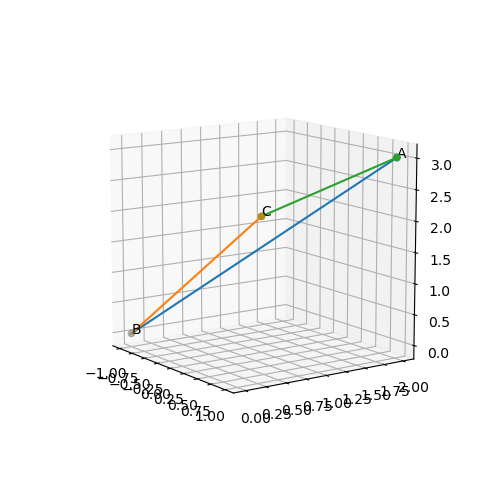
\includegraphics[width=\columnwidth]{chapters/12/10/3/15/figs/Figure_1.png}
   \caption{}
   \label{fig:chapters/12/10/3/15/TriangleABC}
\end{figure}





\item Show that the points $\vec{A}(1,2,7), \vec{B}(2,6,3)$ and $\vec{C}(3,10,-1)$ are collinear.
	\\
	\solution
		\iffalse
\documentclass[journal,12pt,twocolumn]{IEEEtran}
\usepackage{setspace}
\usepackage{gensymb}
\usepackage{xcolor}
\usepackage{caption}
\singlespacing
\usepackage{siunitx}
\usepackage[cmex10]{amsmath}
\usepackage{mathtools}
\usepackage{hyperref}
\usepackage{amsthm}
\usepackage{mathrsfs}
\usepackage{txfonts}
\usepackage{stfloats}
\usepackage{cite}
\usepackage{cases}
\usepackage{subfig}
\usepackage{longtable}
\usepackage{multirow}
\usepackage{enumitem}
\usepackage{mathtools}
\usepackage{listings}
\usepackage{tikz}
\usetikzlibrary{shapes,arrows,positioning}
\usepackage{circuitikz}
\let\vec\mathbf
\DeclareMathOperator*{\Res}{Res}
\renewcommand\thesection{\arabic{section}}
\renewcommand\thesubsection{\thesection.\arabic{subsection}}
\renewcommand\thesubsubsection{\thesubsection.\arabic{subsubsection}}

\renewcommand\thesectiondis{\arabic{section}}
\renewcommand\thesubsectiondis{\thesectiondis.\arabic{subsection}}
\renewcommand\thesubsubsectiondis{\thesubsectiondis.\arabic{subsubsection}}
\hyphenation{op-tical net-works semi-conduc-tor}

\lstset{
language=Python,
frame=single, 
breaklines=true,
columns=fullflexible
}
\begin{document}
\theoremstyle{definition}
\newtheorem{theorem}{Theorem}[section]
\newtheorem{problem}{Problem}
\newtheorem{proposition}{Proposition}[section]
\newtheorem{lemma}{Lemma}[section]
\newtheorem{corollary}[theorem]{Corollary}
\newtheorem{example}{Example}[section]
\newtheorem{definition}{Definition}[section]
\newcommand{\BEQA}{\begin{eqnarray}}
\newcommand{\EEQA}{\end{eqnarray}}
\newcommand{\define}{\stackrel{\triangle}{=}}
\newcommand{\myvec}[1]{\ensuremath{\begin{pmatrix}#1\end{pmatrix}}}
\newcommand{\mydet}[1]{\ensuremath{\begin{vmatrix}#1\end{vmatrix}}}
\bibliographystyle{IEEEtran}
\providecommand{\nCr}[2]{\,^{#1}C_{#2}} % nCr
\providecommand{\nPr}[2]{\,^{#1}P_{#2}} % nPr
\providecommand{\mbf}{\mathbf}
\providecommand{\pr}[1]{\ensuremath{\Pr\left(#1\right)}}
\providecommand{\qfunc}[1]{\ensuremath{Q\left(#1\right)}}
\providecommand{\sbrak}[1]{\ensuremath{{}\left[#1\right]}}
\providecommand{\lsbrak}[1]{\ensuremath{{}\left[#1\right.}}
\providecommand{\rsbrak}[1]{\ensuremath{{}\left.#1\right]}}
\providecommand{\brak}[1]{\ensuremath{\left(#1\right)}}
\providecommand{\lbrak}[1]{\ensuremath{\left(#1\right.}}
\providecommand{\rbrak}[1]{\ensuremath{\left.#1\right)}}
\providecommand{\cbrak}[1]{\ensuremath{\left\{#1\right\}}}
\providecommand{\lcbrak}[1]{\ensuremath{\left\{#1\right.}}
\providecommand{\rcbrak}[1]{\ensuremath{\left.#1\right\}}}
\theoremstyle{remark}
\newtheorem{rem}{Remark}
\newcommand{\sgn}{\mathop{\mathrm{sgn}}}
\newcommand{\rect}{\mathop{\mathrm{rect}}}
\newcommand{\sinc}{\mathop{\mathrm{sinc}}}
\providecommand{\abs}[1]{\left\vert#1\right\vert}
\providecommand{\res}[1]{\Res\displaylimits_{#1}} 
\providecommand{\norm}[1]{\lVert#1\rVert}
\providecommand{\mtx}[1]{\mathbf{#1}}
\providecommand{\mean}[1]{E\left[ #1 \right]}
\providecommand{\fourier}{\overset{\mathcal{F}}{ \rightleftharpoons}}
\providecommand{\ztrans}{\overset{\mathcal{Z}}{ \rightleftharpoons}}
\providecommand{\system}[1]{\overset{\mathcal{#1}}{ \longleftrightarrow}}
\newcommand{\solution}{\noindent \textbf{Solution: }}
\providecommand{\dec}[2]{\ensuremath{\overset{#1}{\underset{#2}{\gtrless}}}}
\let\StandardTheFigure\thefigure
\def\putbox#1#2#3{\makebox[0in][l]{\makebox[#1][l]{}\raisebox{\baselineskip}[0in][0in]{\raisebox{#2}[0in][0in]{#3}}}}
     \def\rightbox#1{\makebox[0in][r]{#1}}
     \def\centbox#1{\makebox[0in]{#1}}
     \def\topbox#1{\raisebox{-\baselineskip}[0in][0in]{#1}}
     \def\midbox#1{\raisebox{-0.5\baselineskip}[0in][0in]{#1}}

\vspace{3cm}
\title{Line Assignment}
\author{Gautam Singh}
\maketitle
\bigskip

\begin{abstract}
    This document contains the solution to Question 16 of Exercise 3 in Chapter
    10 of the class 12 NCERT textbook.
\end{abstract}

\begin{enumerate}
    \item Show that the points $\vec{A} = \myvec{1\\2\\7}$, $\vec{B} = 
    \myvec{2\\6\\3}$, and $\vec{C} = \myvec{3\\10\\-1}$ are collinear.


    \solution 
\fi
		Points $\vec{A}$, $\vec{B}$ and $\vec{C}$ are on a line if
    \begin{align}
        \textrm{rank}\myvec{\vec{A} & \vec{B} & \vec{C}} < 3
        \label{eq:chapters/12/10/3/16rank-collinear}
    \end{align}
    Substituting, we must find the rank of
    \begin{align}
        \vec{M} = \myvec{1&2&3\\2&6&10\\7&3&-1}
    \end{align}
    Using row reduction methods to bring $\mtx{M}$ into row-reduced echelon
    form,
    \begin{align}
        \myvec{1&2&3\\2&6&10\\7&3&-1}&\xleftrightarrow[]{R_2\rightarrow R_2-2R_1}
        \myvec{1&2&3\\0&2&4\\7&3&-1} \\
                &\xleftrightarrow[]{R_3\rightarrow R_3-7R_1}\myvec{1&2&3\\0&2&4\\0&-11&-22} \\
                &\xleftrightarrow[]{R_1\rightarrow R_1-R_2}\myvec{1&0&-1\\0&2&4\\0&-11&-22} \\
                &\xleftrightarrow[]{R_3\rightarrow R_3+\frac{11}{2}R_2}\myvec{1&0&-1\\0&2&4\\0&0&0}
                \label{eq:chapters/12/10/3/16row-red}
    \end{align}
    Clearly, the rank of $\mtx{M}$ is 2, and hence the given points are 
    collinear. 
    Fig. \ref{fig:chapters/12/10/3/163d-line}  verifies that the three points are indeed 
    collinear as claimed.
    \begin{figure}[!ht]
        \centering
        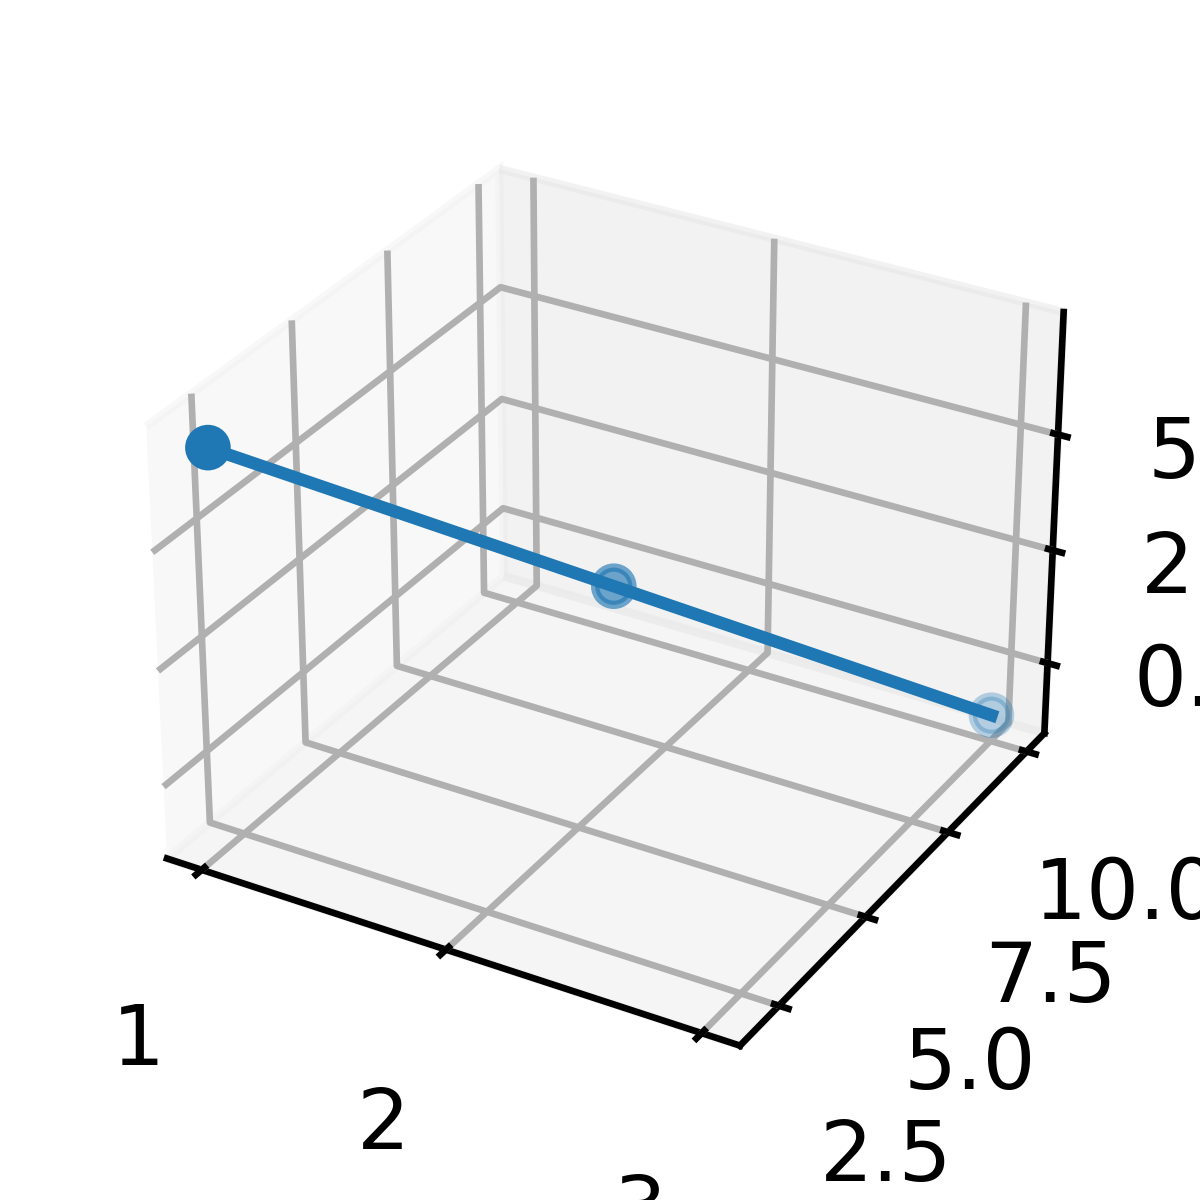
\includegraphics[width=\columnwidth]{chapters/12/10/3/16/figs/line_3d.png}
        \caption{Points $\vec{A}$, $\vec{B}$ and $\vec{C}$ are collinear.}
        \label{fig:chapters/12/10/3/163d-line}
    \end{figure}

\item Show that the vectors $2\hat{i}-\hat{j}+\hat{k},\hat{i}-3\hat{j}-5\hat{k}$ and  $3\hat{i}-4\hat{j}-4\hat{k}$ from the vertices of a right angled triangle.
	\\
	\solution
		\iffalse
\documentclass[journal,12pt,twocolumn]{IEEEtran}
\usepackage{setspace}
\usepackage{gensymb}
\singlespacing
\usepackage[cmex10]{amsmath}
\usepackage{amsthm}
\usepackage{mathrsfs}
\usepackage{txfonts}
\usepackage{stfloats}
\usepackage{bm}
\usepackage{cite}
\usepackage{cases}
\usepackage{subfig}
\usepackage{longtable}
\usepackage{multirow}
\usepackage{enumitem}
\usepackage{mathtools}
\usepackage{steinmetz}
\usepackage{tikz}
\usepackage{circuitikz}
\usepackage{verbatim}
\usepackage{tfrupee}
\usepackage[breaklinks=true]{hyperref}
\usepackage{tkz-euclide}
\usetikzlibrary{calc,math}
\usepackage{listings}
    \usepackage{color}                                            %%
    \usepackage{array}                                            %%
    \usepackage{longtable}                                        %%
    \usepackage{calc}                                             %%
    \usepackage{multirow}                                         %%
    \usepackage{hhline}                                           %%
    \usepackage{ifthen}                                           %%
  %optionally (for landscape tables embedded in another document): %%
    \usepackage{lscape}     
\usepackage{multicol}
\usepackage{chngcntr}
\DeclareMathOperator*{\Res}{Res}
\renewcommand\thesection{\arabic{section}}
\renewcommand\thesubsection{\thesection.\arabic{subsection}}
\renewcommand\thesubsubsection{\thesubsection.\arabic{subsubsection}}

\renewcommand\thesectiondis{\arabic{section}}
\renewcommand\thesubsectiondis{\thesectiondis.\arabic{subsection}}
\renewcommand\thesubsubsectiondis{\thesubsectiondis.\arabic{subsubsection}}

% correct bad hyphenation here
\hyphenation{op-tical net-works semi-conduc-tor}
\def\inputGnumericTable{}                                 %%

\lstset{
frame=single, 
breaklines=true,
columns=fullflexible
}

\begin{document}


\newtheorem{theorem}{Theorem}[section]
\newtheorem{problem}{Problem}
\newtheorem{proposition}{Proposition}[section]
\newtheorem{lemma}{Lemma}[section]
\newtheorem{corollary}[theorem]{Corollary}
\newtheorem{example}{Example}[section]
\newtheorem{definition}[problem]{Definition}
\newcommand{\BEQA}{\begin{eqnarray}}
\newcommand{\EEQA}{\end{eqnarray}}
\newcommand{\define}{\stackrel{\triangle}{=}}

\bibliographystyle{IEEEtran}
\providecommand{\mbf}{\mathbf}
\providecommand{\pr}[1]{\ensuremath{\Pr\left(#1\right)}}
\providecommand{\qfunc}[1]{\ensuremath{Q\left(#1\right)}}
\providecommand{\sbrak}[1]{\ensuremath{{}\left[#1\right]}}
\providecommand{\lsbrak}[1]{\ensuremath{{}\left[#1\right.}}
\providecommand{\rsbrak}[1]{\ensuremath{{}\left.#1\right]}}
\providecommand{\brak}[1]{\ensuremath{\left(#1\right)}}
\providecommand{\lbrak}[1]{\ensuremath{\left(#1\right.}}
\providecommand{\rbrak}[1]{\ensuremath{\left.#1\right)}}
\providecommand{\cbrak}[1]{\ensuremath{\left\{#1\right\}}}
\providecommand{\lcbrak}[1]{\ensuremath{\left\{#1\right.}}
\providecommand{\rcbrak}[1]{\ensuremath{\left.#1\right\}}}
\theoremstyle{remark}
\newtheorem{rem}{Remark}
\newcommand{\sgn}{\mathop{\mathrm{sgn}}}
\providecommand{\abs}[1]{\left\vert#1\right\vert}
\providecommand{\res}[1]{\Res\displaylimits_{#1}} 
\providecommand{\norm}[1]{\left\lVert#1\right\rVert}
\providecommand{\mtx}[1]{\mathbf{#1}}
\providecommand{\mean}[1]{E\left[ #1 \right]}
\providecommand{\fourier}{\overset{\mathcal{F}}{ \rightleftharpoons}}
\providecommand{\system}{\overset{\mathcal{H}}{ \longleftrightarrow}}
\newcommand{\solution}{\noindent \textbf{Solution: }}
\newcommand{\cosec}{\,\text{cosec}\,}
\providecommand{\dec}[2]{\ensuremath{\overset{#1}{\underset{#2}{\gtrless}}}}
\newcommand{\myvec}[1]{\ensuremath{\begin{pmatrix}#1\end{pmatrix}}}
\newcommand{\mydet}[1]{\ensuremath{\begin{vmatrix}#1\end{vmatrix}}}
\numberwithin{equation}{subsection}
\makeatletter
\@addtoreset{figure}{problem}
\makeatother

\let\StandardTheFigure\thefigure
\let\vec\mathbf
\renewcommand{\thefigure}{\theproblem}



\def\putbox#1#2#3{\makebox[0in][l]{\makebox[#1][l]{}\raisebox{\baselineskip}[0in][0in]{\raisebox{#2}[0in][0in]{#3}}}}
     \def\rightbox#1{\makebox[0in][r]{#1}}
     \def\centbox#1{\makebox[0in]{#1}}
     \def\topbox#1{\raisebox{-\baselineskip}[0in][0in]{#1}}
     \def\midbox#1{\raisebox{-0.5\baselineskip}[0in][0in]{#1}}

\vspace{3cm}


\title{Assignment 1}
\author{Jaswanth Chowdary Madala}





% make the title area
\maketitle

\newpage

%\tableofcontents

\bigskip

\renewcommand{\thefigure}{\theenumi}
\renewcommand{\thetable}{\theenumi}


\begin{enumerate}

\item Show that the vectors $2\hat{i}-\hat{j}+\hat{k}$, $\hat{i}-3\hat{j}-5\hat{k}$ and $3\hat{i}-4\hat{j}-4\hat{k}$ form the vertices of a right angled triangle.
\fi
Let
\begin{align}
\vec{A} = \myvec{2\\-1\\1}, \, \vec{B} = \myvec{1\\-3\\-5}, \, \vec{C}=\myvec{3\\-4\\-4} 
\end{align}
 Form the matrix 
\begin{align}
\myvec{\vec{A}&\vec{B}&\vec{C}} = \myvec{2&1&3\\-1&-3&-4\\1&-5&-4}\\
\xleftrightarrow [R_2 \leftarrow R_2+\frac{1}{2}R_1]{R_3 \leftarrow R_3-\frac{1}{2}R_1} \\
\myvec{2&1&3\\ \\0&-\dfrac{5}{2}&-\dfrac{5}{2}\\\\0&-\dfrac{11}{2}&-\dfrac{11}{2}}\\
\xleftrightarrow[]{R_3 \leftarrow R_3-\frac{11}{5}R_2}\\
\myvec{2&1&3\\ \\0&-\dfrac{5}{2}&-\dfrac{5}{2}\\\\0&0&0},
\end{align}
the rank of the matrix is 2 and the points are in 3-Dimensional space, so the points $\vec{A},\vec{B},\vec{C}$ form a triangle.
\begin{enumerate}
\item checking whether the triangle is right angled at $\vec{A}$
\begin{align}
\vec{B}-\vec{A} &= \myvec{-1\\-2\\-6} \\
\vec{C}-\vec{A} &= \myvec{1\\-3\\-5} \\
\brak{\vec{B}-\vec{A}}^{\top}\brak{\vec{C}-\vec{A}} &= \myvec{-1&-2&-6}\myvec{1\\-3\\-5} = 35
\neq 0
\end{align}
The triangle is not right angled at $\vec{A}$.
%
\item checking whether the triangle is right angled at $\vec{B}$
\begin{align}
\vec{A}-\vec{B} &= \myvec{1\\2\\6} \\
\vec{C}-\vec{B} &= \myvec{2\\-1\\1} 
\end{align}
\begin{align}
\brak{\vec{A}-\vec{B}}^{\top}\brak{\vec{C}-\vec{B}} &= \myvec{1&2&6}\myvec{2\\-1\\1} = 6
\neq 0
\end{align}
The triangle is not right angled at $\vec{B}$.
%
\item checking whether the triangle is right angled at $\vec{C}$
\begin{align}
\vec{A}-\vec{C} &= \myvec{-1\\3\\5} \\
\vec{B}-\vec{C} &= \myvec{-2\\1\\-1} \\
\brak{\vec{A}-\vec{C}}^{\top}\brak{\vec{B}-\vec{C}} &= \myvec{-1&3&5}\myvec{-2\\1\\-1} = 0\\
\end{align}
Hence the triangle is right angled at $\vec{C}$.
\end{enumerate}





\item If $\overrightarrow {a}$ is a nonzero vector of magnitude 'a' and $\lambda$ a nonzero scalar , then $\lambda\overrightarrow {a}$ is unit vector if

\begin{enumerate} 
\item $\lambda=1$ 
\item $\lambda=-1$
\item $a=\abs{\lambda}$
\item $a=1/\abs{\lambda}$  
\end{enumerate}
\iffalse
\item If $\overrightarrow {a}=2\hat{i}+2\hat{j}3\hat{k},\overrightarrow {b}=\hat{-i}+2\hat{j}+\hat{k}$ and $\overrightarrow {c}=3\hat{i}+\hat{j}$ are such that $\overrightarrow {a}+\lambda\overrightarrow {b}$ is perpendicular to $\overrightarrow {c}$,then find the value of $\lambda$.
	\\
		\iffalse
\documentclass[12pt]{article}
\usepackage{graphicx}
\usepackage{amsmath}
\usepackage{mathtools}
\usepackage{gensymb}

\newcommand{\mydet}[1]{\ensuremath{\begin{vmatrix}#1\end{vmatrix}}}
\providecommand{\brak}[1]{\ensuremath{\left(#1\right)}}
\providecommand{\norm}[1]{\left\lVert#1\right\rVert}
\newcommand{\solution}{\noindent \textbf{Solution: }}
\newcommand{\myvec}[1]{\ensuremath{\begin{pmatrix}#1\end{pmatrix}}}
\let\vec\mathbf

\begin{document}
\begin{center}
\textbf\large{CHAPTER-10 \\ VECTOR ALGEBRA}

\end{center}
\section*{Excercise 10.3}

Q10.If $\vec{a} = 2\hat{i}+2\hat{j}+3\hat{k}, \vec{b} = -\hat{i}+2\hat{j}+\hat{k} \text{ and } \vec{c} = 3\hat{i}+\hat{j}$ are such that $\vec{a}+\lambda \vec{b}$ is perpendicular to $\vec{c}$, then find the value of $\lambda$.
\fi
\solution
Given that
\begin{align}
	(\vec{a}+\lambda \vec{b})^{\top} \vec{c} &= 0\\
\implies \vec{a}^{\top}\vec{c}+\lambda \vec{b}^{\top}\vec{c}&=0\\
\implies 	\lambda \vec{b}^{\top}\vec{c}&=-\vec{a}^{\top}\vec{c}\\
\implies 	\lambda(\vec{b}^{\top}\vec{c})(\vec{b}^{\top}\vec{c})^{-1}&=-(\vec{a}^{\top}\vec{c})(\vec{b}^{\top}\vec{c})^{-1}\\
\implies 	\lambda&=-(\vec{a}^{\top}\vec{c})(\vec{b}^{\top}\vec{c})^{-1}
\end{align}
Now substituting the values
\begin{align}
	\vec{a}^{\top}\vec{c}&=\myvec{2&2&3} \myvec{3\\1\\0} = 8\\
	\vec{b}^{\top}\vec{c}&=\myvec{-1&2&1} \myvec{3\\1\\0} = -1,
\end{align}
\begin{align}
	\lambda&=-(\vec{a}^{\top}\vec{c})(\vec{b}^{\top}\vec{c})^{-1}\\
	&=-(8)(-1)^{-1}\\
	&=8
\end{align}



\item Show that $\abs {\overrightarrow {a}}\overrightarrow {b}+\abs{\overrightarrow {b}}\overrightarrow {a}$ is perpendicular to $\abs{\overrightarrow {a}} \overrightarrow {b}-\abs{\overrightarrow {b}} \overrightarrow {a}$, for any two nonzero vectors $\overrightarrow {a}$ and $\overrightarrow {b}$.
\item If $\overrightarrow {a}.\overrightarrow {a}$=0 and $\overrightarrow {a}.\overrightarrow {b}$=0, then what can be conculded about the vector $\overrightarrow {b}$?
\item If $\overrightarrow {a},\overrightarrow {b},\overrightarrow {c}$ are unit vectors such that $\overrightarrow {a}+\overrightarrow {b}+\overrightarrow {c}=\overrightarrow {0}$, find the value of $\overrightarrow {a}.\overrightarrow {b}+\overrightarrow {b}.\overrightarrow {c}+\overrightarrow {c}.\overrightarrow {a}$.
\item If either vector $\overrightarrow {a}=0$ or $\overrightarrow {b}=0$, then $\overrightarrow {a}.\overrightarrow {b}$=0. But the converse need not be true .Justify your answer with an example.
\item If the vertices A,B,C of a triangle ABC are (1,2,3),(-1,0,0)(0,1,2), respectively , then find  $\angle{ABC}. [\angle{ABC}$ is the angle between the vectors $\overrightarrow{BA}$ and $\overrightarrow{BC}$].
\item show that the points A(1,2,7),B(2,6,3)and C(3,10,-1) are collinear.
\item show that the vectors $2\hat{i}-\hat{j}+\hat{k},\hat{i}-3\hat{j}-5\hat{k}$ and  $3\hat{i}-4\hat{j}-4\hat{k}$ from the vertices of a right angled triangle.
\item If $\overrightarrow {a}$ is a nonzero vector of magnitude 'a' and $\lambda$ a nonzero scalar , then $\lambda\overrightarrow {a}$ is unit vector if

\begin{enumerate} 
\item $\lambda=1$ 
\item $\lambda=-1$
\item $a=\abs{\lambda}$
\item $a=1/\abs{\lambda}$  
\end{enumerate}
\fi

\end{enumerate}

